\documentclass[12pt]{article}
\usepackage[T1]{fontenc} 
\usepackage[portuguese]{babel}
\usepackage{hyphenat}
% use se você precisar forçar a separação de sílabas em quebra de linha
\hyphenation{mate-mática recu-perar}
\usepackage{graphicx}
\graphicspath{images/}
\usepackage{csquotes}
\usepackage{subfiles}
\usepackage{amsmath}
\usepackage{csvsimple} 
\usepackage{geometry}

\geometry{
    a4paper,
    left=3cm,
    top = 3cm,
    right=2cm,
    bottom=2cm
}
\setlength{\parindent}{4em}
%\setlength{\parskip}{1em}
\renewcommand{\baselinestretch}{1.5}

\usepackage[dvipsnames]{xcolor}
\definecolor{alert}{RGB}{201, 58, 128}
\setlength {\marginparwidth }{2cm} 
\usepackage[colorinlistoftodos]{todonotes}
\usepackage{comment}
\usepackage{subcaption}
\DeclareUnicodeCharacter{0301}{*************************************}
\usepackage{enumitem}
%% CSS: mudando o gerenciador de bibliografia para biblatex para contornar 
% alguns problemas. Adendo: a compilação no overleaf ficou muito instável 
% e por alguma razão não imprime a seção de bibliografia no final, apesar
% de colocar as anotações ao longo do texto. Voltando ao bibtex no momento (5/9/2024)
%\usepackage{biblatex}
%\addbibresource{ref.bib}

\title{TÍTULO}
\author{autor}

\begin{document}

% CAPA
\thispagestyle{empty}

    
    \begin{flushright}
        \begin{huge}
            \textbf{RELATÓRIO}\\[3,5cm]
        \end{huge}
%% CSS: Podemos usar um título mais genérico agora e depois discutir um definitivo
{\bf \LARGE  CLASSIFICAÇÃO DE GLAUCOMA EM IMAGENS DE FUNDO DE OLHO COM APRENDIZAGEM PROFUNDA}

\bigskip
        
        Leandro Zangirolami Trovões (Orientando)\\
        Carlos da Silva dos Santos (Orientador)\\
        Universidade Federal do ABC\\[5,5cm]
    \end{flushright}

    \vfill
    
    \begin{center}
        Santo André,\\
        Setembro de 2024
    \end{center}
    
    \newpage
\bigskip

\begin{center}
\noindent{\bf \Large Resumo}
\end{center}

\begin{quote}
O glaucoma é a principal causa de cegueira irreversível no mundo, podendo atingir até 111,8 milhões de pessoas até 2040. Caracterizada pelo dano progressivo ao nervo ótico, a doença não tem cura e é assintomática em seus estágios iniciais, tornando o diagnóstico precoce essencial para retardar ou prevenir sua progressão. O exame de fundoscopia é uma das principais formas de identificar a doença, no qual é possível observar alterações características do glaucoma. Recentemente, técnicas de aprendizagem profunda têm sido aplicadas no diagnóstico de glaucoma em imagens de fundo de olho. O emprego de diferentes arquiteturas de redes neurais convolucionais tem apresentado resultados significativos. Contudo, a limitação da disponibilidade de imagens para treinamento e a falta de interpretabilidade são frequentemente apontadas como limitações.

Esse trabalho propõe o desenvolvimento de uma rede neural convolucional para a identificação de glaucoma em imagens de fundo de olho, focando na interpretabilidade dos resultados. Utilizaremos o banco de dados JustRAIGS, que inclui anotações adicionais que justificam a classificação atribuída as imagens pelos avaliadores.
\end{quote}

\begin{center}
Santo André, setembro de 2024
\end{center}

\newpage
\bigskip

\section{Introdução}
\label{sec:introducao}

%% CSS: usar o ~ antes do \cite impede que o latex quebre linha entre 
%       o texto e a anotação
Principal causa de cegueira irreversível no mundo~\cite{steinmetz_causes_2021}, o glaucoma é uma doença sem cura, caracterizada pelo dano progressivo ao nervo ótico~\cite{who_2019}. Estima-se que, em 2020, 3,6 milhões de pessoas com 50 anos ou mais já tenham perdido a visão para o Glaucoma~\cite{steinmetz_causes_2021} e um estudo de 2014 ainda projeta que 111.8 milhões de pessoas sejam afetadas pela doença no ano de 2040.~\cite{tham_global_2014}.

Assintomática em seus estágios iniciais, conforme avança, a doença causa perda de visão periférica e, se não for tratada, pode levar a perda total da visão. O tratamento pode retardar ou prevenir a progressão, mas depende de um diagnóstico precoce, geralmente antes mesmo dos primeiros sintomas~\cite{who_2019}.

\begin{comment}
O tratamento consiste em reduzir a pressão intra-ocular e 

fatores de risco: idade, histórico familiar

OMS: General population screening for glaucoma is not currently
considered to be cost-effective in most settings (63). Therefore,
routine eye examinations are recommended for high-risk individuals
as early detection is essential for the protection of visual function. 
\end{comment}

Uma das formas de identificar a presença de glaucoma é por meio da fundoscopia ou exame de fundo de olho, no qual é possível observar alterações características, muitas vezes antes mesmo que a perda de visão se torne detectável~\cite{weinreb_2004}. Um exemplo de imagem obtida nesse exame é apresentado na Figura~\ref{fig:fundus}.

A principal característica observada ao analisar o fundo de olho é o tamanho da escavação em relação ao tamanho do disco ótico do paciente, ambos destacados na Figura~\ref{fig:disk}. O disco ótico é a região em que as células da retina se convergem para formar o nervo ótico. Essa convergência forma uma depressão ao centro do disco, chamada de escavação (em inglês conhecido como \emph{optic cup}). O anel neurorretiniano é a região que envolve a escavação. A razão entre o tamanho do disco e da escavação é conhecida como razão disco-copo (em inglês \emph{cup-to-disk ratio}) e seu valor acima do normal é um indicativo do dano causado pela doença ~\cite{weinreb_2004}. % posso também citar weinreb_2016 para essa última afirmação

\begin{figure}[htb]
 \centering
 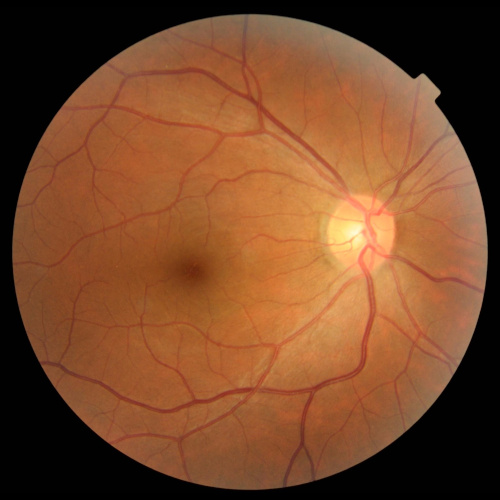
\includegraphics[width=0.3\textwidth]{images/TRAIN000004_cut.JPG}
 \caption{Imagem de fundo de olho. Obtida do banco de dados JustRAIGS.}
 \label{fig:fundus}
\end{figure}

\begin{comment}
Dentre as características observadas estão: 1, 2, 3, 4 e 5. cite{"Five rules to evaluate the optic disc and retinal nerve fiber layer for glaucoma"}

A capacidade da inteligência artificial em --- atrai seu uso na medicina. cite{alguem}

uso de IA com imagens médicas aumentou\\


fazer a avaliação manual gera divergência entre médicos, falta de padronização -> podemos fazer de forma automática
\end{comment}

\begin{comment}
da pra falar que médicas acreditam no potencial da IA
tem essa pesquisa aqui mas me parece muito restrita: só australia e nova zelancia e só com  trainees
...médicos acreditam que IA vai melhorar o trabalho deles... \cite{scheetz_survey_2021}
\end{comment}

Recentemente, diversas técnicas de aprendizagem profunda vem sendo aplicadas no diagnóstico de doenças com base em imagens de fundo de olho, inclusive para o glaucoma~\cite{li_review_2021}. Para possibilitar o desenvolvimento desses modelos, bancos de dados com imagens de fundo de olho classificadas por oftalmologistas foram criados e alguns deles disponibilizados publicamente, como o RIGA~\cite{riga}, ORIGA~\cite{origa}, RIM-ONE DL~\cite{RIMONEDL} e JustRAIGS~\cite{justraigs}. Um quadro resumo com alguns bandos de dados é apresentado na Tabela~\ref{tab:datasets}. 

\begin{figure}[htb]
 \centering
 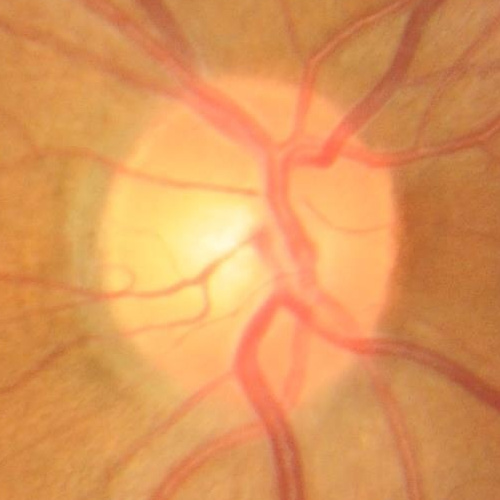
\includegraphics[width=0.3\textwidth]{images/disk.jpg}
 \caption{Disco ótico em destaque. Obtida do banco de dados JustRAIGS.}
 \label{fig:disk}
\end{figure}

Trabalhos anteriores conseguiram realizar a classificação de imagens entre glaucoma e não glaucoma utilizando diferentes técnicas. Noronha et al. (2014) utilizou cumulantes de alta ordem para identificar glaucoma em 272 imagens de fundo de olho obtidas por conta própria, obtendo acurácia de 84.72\% \cite{noronha2014hoc}. Chen et al. (2015) implementou uma rede neural convolucional, contendo seis camadas sendo quatro convolucionais e 2 totalmente conectadas, e a treinou em dois bancos de dados privados, obtendo de resultado os valores de área sobre curva (AUC) 0.831 e 0.887 \cite{chen2015cnn}. Liu et al. (2019) desenvolveu uma rede convolucional baseada na arquitetura ResNet e a treinou com 241.032 imagens, obtendo uma AUC de 0.996 \cite{liu_cnn_2019}. Um quadro resumo com estes e outros trabalhos é apresentado na Tabela~\ref{tab:trabalhos}.

Em seu estudo de revisão, a respeito do uso de aprendizagem profunda em imagens de fundo de olho, Li et al. \cite{li_review_2021} aponta como algumas das limitações e áreas para melhorias futuras a baixa disponibilidade de dados anotados com qualidade e a falta de interpretabilidade dos resultados, característica inerente à aprendizagem profunda.

O banco de dados JustRAIGS, além de incluir anotações entre referenciável para glaucoma ou não para 101.422 imagens, também possui 10 anotações adicionais, para sinais observados pelos avaliadores, que justifiquem a escolha da imagem como referenciável para glaucoma, naquelas assim marcadas \cite{justraigs_article}.

O presente trabalho procura explorar o uso de redes neurais convolucionais no problema de classificação do glaucoma em imagens de fundo olho, além de investigar o uso das anotações adicionais presentes no JustRAIGS como forma de auxiliar na interpretabilidade dos resultados produzidos pelos modelos.

O restante do texto é organizado da seguinte maneira: em primeiro lugar, apresentamos os objetivos deste trabalho na Seção~\ref{sec:objetivo} e, em seguida, apresentamos na Seção~\ref{sec:schedule} o plano de trabalho proposto.

\begin{comment}
DESCONSIDERAR ESSE BLOCO

usando redes neurais\\
e até mesmo técnicas de processamento de sinais\cite{Noronha2014}

porem:
\begin{itemize}
 \item datasets limitados (agora temos um de 100k imagens) e alguns são privados
 \item falta de justificativa, blackbox ~\cite{li_review_2021} 7.2.5, usar features adicionais para explicar decisão
\end{itemize}

suposições que precisam ser sustentadas:\\
1- razão OD e OC é a melhor forma de identificar glaucoma\\
2- CNN é melhor de que calcular a razão ente OD e OC: [Chen, 2015] afirma mas não sustenta. Cita [3]\\

2) Diaz-Pinto, 2019: usando CNN não precisa fazer segmentação perfeita do OD e do OC
"Important limitations of the methods that are based on handcrafted characteristics (CDR, Area Cup/Disc ratio (ACDR), vessel kinks and ISNT rule) is the significant disagreement in estimating them even between expert human graders. For that reason, new algorithms have been focused on automatic feature extraction such as the data-driven methods [3] and convolutional neural networks (CNNs)."\\
Menciona alguns trabalhos que foram pela abordagem da segmentação e os resultados obtidos.

investigar:
Chen, 2015: 17 5 6 14, 2, 12, 13\\
Noronha, 2014: 9, 16, 17, 18

\end{comment}

\begin{table}[htb]
    \centering
    \begin{tabular}{|c|c|c|}
    \hline
    Nome & Nº de imagens & Ano de publicação \\
    \hline
    ORIGA & 650 & 2010 \\
    \hline
    DRISHTI-GS1 & 101 & 2015 \\
    \hline
    RIGA & 750 & 2018 \\
    \hline
    RIM-ONE DL & 485 & 2020 \\
    \hline
    REFUGE & 1200 & 2020 \\
    \hline
    JustRAIGS & 101.442 & 2024 \\
    \hline
    \end{tabular}
    \caption{Bancos de dados para avaliação de glaucoma}
    \label{tab:datasets}
\end{table}

\begin{table}[htb]
    \centering
    % o formato p (de parágrafo) permite ajustar largura e causa quebra de linha
    \begin{tabular}{|l|l|p{3cm}|c|c|}
    \hline
    Artigo                                      & Método      & Banco de dados                 & ACC   & AUC   \\
    \hline
    Noronha et al. (2014) \cite{noronha2014hoc} & Cumulantes  & Privado com 272 imagens        & 0.847 &  -    \\
    \hline
    Chen et al. (2015) \cite{chen2015cnn}       & CNN própria & ORIGA                          & -     & 0.831 \\
    \hline
    Chen et al. (2015) \cite{chen2015cnn}       & CNN própria & ORIGA, SCES                    & -     & 0.887 \\
    \hline
    Ferreira et al. (2018) \cite{ferreira_cnn_2018} & U-Net   & RIM-ONE, DRISHTI-GS, DRIONS-DB & 1     & 1     \\
    \hline
    Liu et al. (2019) \cite{liu_cnn_2019}       & ResNet      & Privado com 241.032 imagens    & 0.996 & -     \\
    \hline
    Nawaz et al. (2022) \cite{nawaz_efficient_2022} & EfficientNet-B0 & ORIGA                  & 0.972 & 0.979 \\
    \hline
    \end{tabular}
    \caption{Trabalhos anteriores e resultados obtidos}
    \label{tab:trabalhos}
\end{table}

\bigskip

\section{Objetivos}
\label{sec:objetivo}

\begin{comment}
Objetivos: (devem ser mensuráveis, chegar no final do trabalho e dizer que atingiu)
  criar modelo que seja interpretável
secundário:
 - "comparar modelos quanto à interpretabilidade"
 - determinar metodologia para comparar interpretabilidade
\end{comment}

O objetivo geral deste trabalho é realizar a identificação de glaucoma em imagens de fundo de olho, utilizando um modelo de aprendizagem profunda, que seja interpretável.

Os objetivos específicos são:
\begin{itemize}
 \item realizar a segmentação do disco ótico, a região de interesse (ROI)
 % revisão da literatura sobre diferentes arquiteturas de forma a organizar conhecimento
\end{itemize}


\begin{comment}
Resultados parciais

O disco ótico e seu entorno representam uma pequena porção da imagem de fundo de olho, porém as principais alterações observadas pelos oftalmologistas se encontram nessa área (missing citation). Como tentativa de (melhorar a performance | "facilitar a vida") do classificador a ser desenvolvido, vamos inicialmente segmentar o disco ótico e recortar a imagem em seu entorno, antes de envia-la ao classificador. 


\end{comment}

\bigskip

\section{Plano de trabalho}
\label{sec:schedule}

O plano de trabalho proposto, para o segundo de três períodos, contém as seguintes etapas:
\begin{itemize}
    \item \textbf{Refinar segmentador:} continuar o treinamento do segmentador do disco ótico, a região de interesse (ROI)
    \item \textbf{Avaliar segmentador:} comparar a performance do segmentador com outros disponíveis publicamente
    \item \textbf{Determinar conjunto de dados:} analisar distribuição de classes do JustRAIGS e avaliar possível uso de outros bancos de dados
    \item \textbf{Definir arquitetura do classificador:} estudar e avaliar as arquiteturas existentes para o classificador, com foco na interpretabilidade
    \item \textbf{Definir protocolo de treinamento e avaliação}: definir a forma que será feito o treinamento, função de perda e métricas de avaliação
    \item \textbf{Implementar classificador}
    \item \textbf{Treinar classificador}
    \item \textbf{Revisão de fundamentos:} estudo e revisão de fundamentos teóricos
    \item \textbf{Escrita do relatório}
\end{itemize}

A figura~\ref{fig:crono} apresenta o cronograma proposto com as etapas definidas acima.

\begin{figure}[htb]
 \centering
 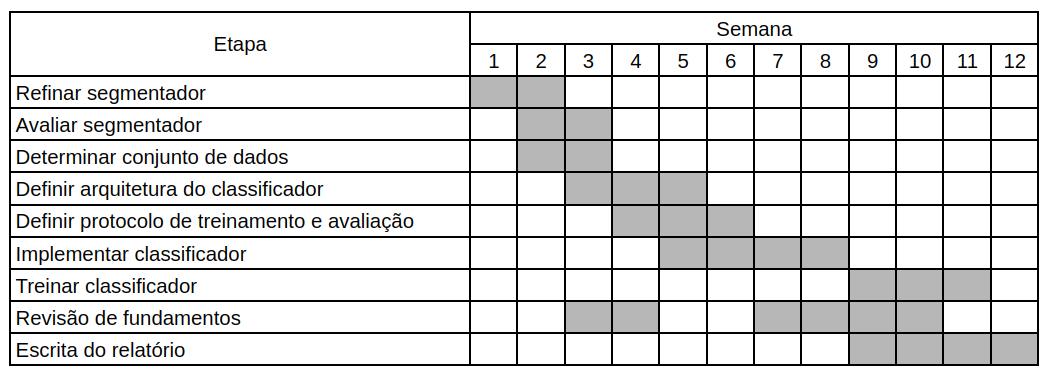
\includegraphics[width=1.0\textwidth]{images/crono_q2.png}
 \caption{Cronograma de execução da proposta}
 \label{fig:crono}
\end{figure}

\bigskip

\section{Materiais e Métodos}
\label{sec:methodology}

\subsection{Conjunto de dados}
\label{sec:dataset}

Foi escolhido o conjunto de dados JustRAIGS \cite{justraigs} que contém 101.442 imagens de fundo de olho publicamente disponíveis, derivado do conjunto de dados REGAIS – \emph{Rotterdam EyePACS Glaucoma AI Screening} \cite{justraigs_article}. As imagens foram providas pelo EyePACS LLC em Santa Cruz, Califórnia nos EUA enquanto as anotações foram providas pelo Instituto de Oftalmologia de Roterdã (\emph{Rotterdam Ophthalmic Institute}) do \emph{Rotterdam Eye Hospital} em Roterdã nos Países Baixos.

\subsubsection{Análise}
\label{sec:dataset:analysis}
Das 101.442 imagens que o conjunto de dados alega possuir, 19 não foram encontradas, restando 101.423. O conjunto é bastante desbalanceado: dentre todas as imagens, apenas 3.270 receberam anotação final para glaucoma, o que representa aproximadamente 3,22\% ou 1 em cada 31.

falar de G1, G2 e G3
resolução de conflito
incluir: As análises que seguem são baseadas no resultado obtido por meio deste algoritmo.

Das anotações adicionais, presentes apenas nos casos com anotação final para glaucoma, X é a mais frequente, aparecendo em XX\% das referenciáveis para glaucoma (ou YY\% do total), Y por sua vez é a menos frequente, aparecendo em apenas YY\% (YY\%). É possível observar certas correções entre as anotações adicionais, apresentadas na Figura Z por meio de uma matriz de correlação.

[fig matriz correlação]

\subsubsection{Divisão entre treino e teste}
\label{sec:dataset:split}

\subsection{Segmentação}
\label{sec:segmentation}

YOLO

\subsection{Classificação}
\label{sec:classification}

ResNet50

\subsection{Recursos computacionais}
\label{sec:resources}

Todos os modelos foram implementados em Python com Keras utilizando o TensorFlow v2.18.0 de backend, com exceção do YOLO (Ultralytics) que utiliza o PyTorch. As versões dos pacotes eram: Python 3.10.12, Keras 3.6.0, TensorFlow 2.18.0, Ultralytics 8.3.18.
Os códigos foram executados com o sistema operacional Pop!\_OS 22.04, kernel Linux 6.9.3, tendo instalado o driver da NVIDIA 560.35.03 e as bibliotecas NVIDIA CUDA 12.6 e NVIDIA cuDNN 9.5.1.
O computador estava equipado com um processador Intel i7-10700K, 32 GB de RAM e uma GPU NVIDIA GeForce RTX 3070.

\bigskip

%% LZT: Como fazer para não incluir a lista completa de nomes? [SBB+21] ficou muito grande
%% CSS: Parte da mudança para biblatex; suspendendo por enquanto,
% ver comentário no preâmbulo (5/9/2024)
% \printbibliography
\bibliographystyle{alpha}%{hapalike}
\bibliography{ref.bib}


\end{document}
